\documentclass[%
 %reprint,
  twocolumn,
 %superscriptaddress,
 %groupedaddress,
 %unsortedaddress,
 %runinaddress,
 %frontmatterverbose,
 % preprint,
 showpacs,
 showkeys,
 preprintnumbers,
 %nofootinbib,
 %nobibnotes,
 %bibnotes,
 amsmath,amssymb,
 aps,
 % prl,
  pra,
 % prb,
 % rmp,
 %prstab,
 %prstper,
  longbibliography,
 floatfix,
 %lengthcheck,%
 ]{revtex4-1}

\usepackage{tikz}
\usetikzlibrary{decorations.pathreplacing,decorations.markings}


\tikzset{
  % style to apply some styles to each segment of a path
  on each segment/.style={
    decorate,
    decoration={
      show path construction,
      moveto code={},
      lineto code={
        \path [#1]
        (\tikzinputsegmentfirst) -- (\tikzinputsegmentlast);
      },
      curveto code={
        \path [#1] (\tikzinputsegmentfirst)
        .. controls
        (\tikzinputsegmentsupporta) and (\tikzinputsegmentsupportb)
        ..
        (\tikzinputsegmentlast);
      },
      closepath code={
        \path [#1]
        (\tikzinputsegmentfirst) -- (\tikzinputsegmentlast);
      },
    },
  },
  % style to add an arrow in the middle of a path
  mid arrow/.style={postaction={decorate,decoration={
        markings,
        mark=at position .5 with {\arrow[#1]{stealth}}
      }}},
 % style to add an arrow in 1/4th of a path
  oneforth arrow/.style={postaction={decorate,decoration={
        markings,
        mark=at position .25 with {\arrow[#1]{stealth}}
      }}},
}
\begin{document}
\begin{center}
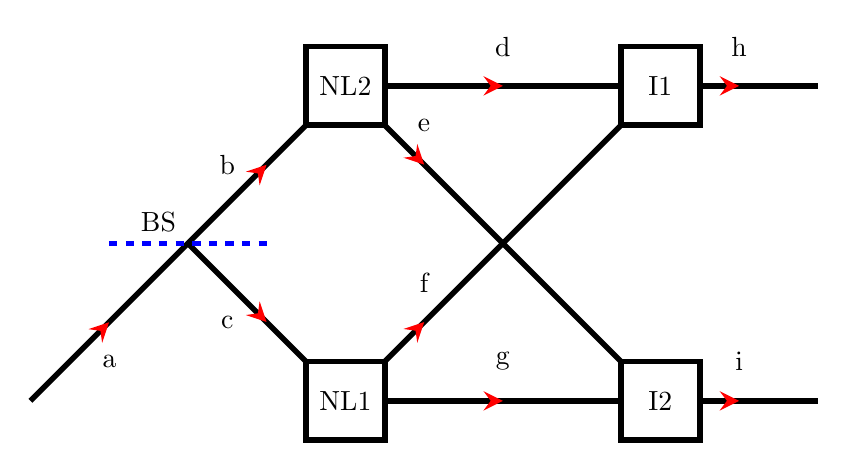
\begin{tikzpicture} [scale=2]

\tikzstyle{every path}=[line width=2pt]

 \path
  (0,0) coordinate(1)
  (1,1) coordinate(2)  % BS
  (2,2) coordinate(3)  % NL1
  (2,0) coordinate(4)  % NL2
  (4,2) coordinate(5)  % I1
  (4,0) coordinate(6)  % I2
  (5,2) coordinate(7)  % h
  (5,0) coordinate(8)  % i
  (0.5,1) coordinate(9)  % BSa
  (1.5,1) coordinate(10)  % BSb
;


\path [draw=black,postaction={on each segment={mid arrow=red}}]  (1) -- (2) -- (3);
\path [draw=black,postaction={on each segment={mid arrow=red}}]  (2) -- (4);
\path [draw=black,postaction={on each segment={mid arrow=red}}]  (3) -- (5);
\path [draw=black,postaction={on each segment={oneforth arrow=red}}]  (3) -- (6);
\path [draw=black,postaction={on each segment={oneforth arrow=red}}]  (4) -- (5);
\path [draw=black,postaction={on each segment={mid arrow=red}}]  (4) -- (6);
\path [draw=black,postaction={on each segment={mid arrow=red}}]  (6) -- (8);
\path [draw=black,postaction={on each segment={mid arrow=red}}]  (5) -- (7);
\path [draw=blue,dashed]  (9) -- (10);
\draw [fill=white] (3) ++(-0.25,-0.25) rectangle node {NL2} ++(0.5,0.5);
\draw [fill=white] (4) ++(-0.25,-0.25) rectangle node {NL1} ++(0.5,0.5);
\draw [fill=white] (5) ++(-0.25,-0.25) rectangle node {I1} ++(0.5,0.5);
\draw [fill=white] (6) ++(-0.25,-0.25) rectangle node {I2} ++(0.5,0.5);
\draw (2) coordinate[label=100:BS];

\node (a) at (0.5,0.25) {a};
\node (b) at (1.25,1.5) {b};
\node (c) at (1.25,0.5) {c};
\node (g) at (3,0.25) {g};
\node (d) at (3,2.25) {d};
\node (e) at (2.5,1.75) {e};
\node (f) at (2.5,0.75) {f};
\node (h) at (4.5,2.25) {h};
\node (i) at (4.5,0.25) {i};

\end{tikzpicture}
\end{center}
\end{document}

 \path [draw=blue,postaction={on each segment={mid arrow=red}}]
  (.2,0) -- (3,1) arc (0:180:1.4 and 1) -- cycle
  (4,1) circle(.8)
  (6,1) ellipse(.5 and 1)
  (0,3) to [bend left] (3,4)
  (4,3) rectangle (6,4)
  ;
